\section{Experiments}\label{sec:exp}
This section empirically evaluates Flow-GRPO's ability to improve flow matching models on three tasks.
% First, in composition generation and text rendring,
% we use rule-based reward models to model the desired behaviors in each task and then  to steer larger models of various scales (Section~\ref{subsec:exp-geneval} \& Section~\ref{subsec:exp-text_rendering}).
% Next, xxx (Section~\ref{subsec:exp-instruction-following}).
(1) Composition Image Generation: This task requires precise object arrangement and attribute control. We report the results on GenEval. (2) Visual Text Rendering: a rule‑based task that evaluates the accurate rendering of the text specified in the prompt. (3) Human Preference Alignment: This task aims to align T2I models with human preferences.


\subsection{Experimental Setup}
\label{sec:exp_setup}
We introduce three tasks, detailing their respective prompts and reward definitions. For hyperparameter details and compute resource specifications, please refer to Appendix~\ref{app:subsubsec:synthetic-hyperp} and Appendix~\ref{app:subsubsec:synthetic-compute}.
% \paragraph{Baselines}
% Together with Flow-GRPO, we benchmark three established alignment methods, each implemented in its stronger online variant, since online updates typically yield better performance \cite{ddpo}.  
% At every training step we generate a group of images whose size matches that used by FlowPO, then apply one of the following update rules:
% \begin{itemize}
% \setlength{\itemindent}{-2em}
%   \item \textbf{Online SFT.} From each batch we select the <prompt, image> pair with the highest reward and perform supervised fine-tuning on these samples.
%   \item \textbf{Online Flow-AWR}~\cite{videoalign,awr}. Flow-AWR align models with reward-weighted likelihood maximization. In the online version we compute a softmax over the rewards in the current group and use the resulting weights to update the model.
%   \item \textbf{Online Flow-DPO}~\cite{videoalign}. Flow-DPO is the flow-matching analogue of DPO. For each batch we select the highest-reward image as the \emph{chosen} sample and the lowest-reward image as the \emph{rejected} sample, then optimise the DPO objective with this pair.
% \end{itemize}


% \subsection{Geneval}\label{subsec:exp-geneval}

% \paragraph{Setup.}
% Geneval assesses a text-to-image model’s ability to handle complex compositional requests, such as object counting, spatial relations, and attribute binding, across six tasks of ascending difficulty.
% We adopt the official evaluation pipeline, which first detects each object’s bounding box and color, then infers pairwise spatial relations. 我们使用geneval提供的构造脚本来构造训练所用的prompt~\footnote{}, 我们进行了严格的测试集过滤，包括'a photo of A and B'和'a photo of B and A'被认为是相同的，也会从训练集中去除
% Rewards are rule-based as follows:
% \begin{itemize}
% \setlength{\itemindent}{-2em}
%   \item \textbf{Counting:} \( r = |N_{\text{generation}} - N_{\text{prompt}}|\, / \,N_{\text{prompt}} \).
%   \item \textbf{Position / Color:} If the object count is correct, we assign a partial reward; the remainder is granted when the predicted position or color is also correct.
% \end{itemize}
% Therefore, the reward is bounded in the range \([0,1]\).


% \subsection{Text Rendering}\label{subsec:exp-text_rendering}
% \paragraph{Setup.}
% The prompt 格式是A sign that says 'Text to Image'. 引号里面是需要rendering的text. 我们使用gpt构造了20k的训练集和1k测试集
% Rewards are rule-based as \( r = |N_{\text{generation}} - N_{\text{prompt}}|\, / \,N_{\text{prompt}} \), where \((N_{\text{generation}}\) is the number of characters detected and \((N_{\text{prompt}}\)
%  is the number of prompt里被双引号包裹的字符
% **Task Selection:** We select three representative tasks:  
% - **Geneval:** A high-level task with rule-based dense rewards, requiring precise object arrangement and attribute control.  
% - **OCR: A high-level task with rule-based rewards, emphasizing text legibility and spatial accuracy.  
% - **Deqa:** A low-level task with VLM-based rewards, focusing on visual question-answering alignment.  
\paragraph{Compositional Image Generation.}\label{subsec:exp-geneval}
GenEval~\cite{geneval} assesses T2I models on complex compositional prompts—like object counting, spatial relations, and attribute binding—across six difficult compositional image generation tasks. We use its official evaluation pipeline, which detects object bounding boxes and colors, then infers their spatial relations. Training prompts are generated using official GenEval scripts, which apply templates and random combinations to construct the prompt dataset. The test set is strictly deduplicated: prompts differing only in object order (e.g., \texttt{"a photo of A and B"} vs. \texttt{"a photo of B and A"}) are treated as identical, and these variants are removed from the training set. Based on the base model's initial accuracy across the six tasks, we set the prompt ratio as \( \texttt{Position}:\texttt{Counting}:\texttt{Attribute Binding}:\texttt{Colors}:\texttt{Two Objects}:\texttt{Single Object} = 7:5:3:1:1:0\).
Rewards are rule-based: (1) \textbf{Counting:} \( r = 1-|N_{\text{gen}} - N_{\text{ref}}| / N_{\text{ref}} \); (2) \textbf{Position / Color:} If the object count is correct, a partial reward is assigned; the remainder is granted when the predicted position or color is also correct.

\paragraph{Visual Text Rendering~\cite{textdiffuser}.}\label{subsec:exp-text_rendering}
Text is common in images such as posters, book covers, and memes, so the ability to place accurate and coherent text inside the generated images is crucial for T2I models.
In our settings, we define an text rendering task, where each prompt follows the template \texttt{``A sign that says ``text''}.
Specifically,
the placeholder \texttt{``text''} is the exact string that should appear in the image.
We use GPT4o to produce 20K training prompts and 1K test prompts. Following \cite{seedream2}, we measure text fidelity with the reward
\(
r = \max (1-N_{\text{e}}/N_{\text{ref}}, 0),
\)
where \( N_{\text{e}} \) is the minimum edit distance
between the rendered text and the target text and \( N_{\text{ref}} \) is the number of characters inside the quotation marks in the prompt. This reward also serves as our metric of text accuracy.


\paragraph{Human Preference Alignment~\cite{kirstain2023pick}.} \label{subsec:exp-human_preference}
This task aims to align T2I models with human preferences. We use \texttt{PickScore}~\cite{kirstain2023pick} as our reward model, which is based on large-scale human annotated pairwise comparisons of images generated from the same prompt. For each image and prompt pair, \texttt{PickScore} provides an overall score that evaluates multiple criteria, such as the alignment of the image with the prompt and its visual quality.

\paragraph{Image Quality Evaluation Metric.}
% Because the T2I model is trained to maximise a predefined reward signal in RL, it is susceptible to reward hacking—situations in which the numerical reward rises but the quality or diversity of the generated images declines. This study aims to make online RL truly effective for T2I generation without compromising quality or diversity. To detect potential reward hacking beyond task-specific accuracy, we evaluate four automatic image quality metrics (i.e., Aesthetic score~\cite{schuhmann2022laion}, DeQA score~\cite{deqa}, ImageReward~\cite{xu2024imagereward}, UnifiedReward~\cite{wang2025unified}). See Appendix~\ref{app:subsubsec:quality_metric} for more details. Moreover, all metrics are evaluated on DrawBench~\cite{drawbench}, a comprehensive and challenging benchmark with diverse prompts for T2I models.
Since the T2I model is trained to maximize a predefined reward, it is vulnerable to reward hacking, where the reward increases but image quality or diversity declines. This study aims to make online RL effective for T2I generation without noticeably compromising quality or diversity. To detect reward hacking beyond task-specific accuracy, we evaluate four automatic image quality metrics: Aesthetic Score~\cite{schuhmann2022laion}, DeQA~\cite{deqa}, ImageReward~\cite{xu2024imagereward}, and UnifiedReward~\cite{wang2025unified} (see Appendix~\ref{app:subsubsec:quality_metric} for details). All metrics are computed on DrawBench~\cite{drawbench}, a comprehensive benchmark with diverse prompts for T2I models.
\begin{table*}[t]
    \centering
    \caption{{\bf GenEval Result.} 
Best scores are in \colorbox{pearDark!20}{blue}, second-best in \colorbox{color_green}{green}. Results for models other than SD3.5-M are from~\cite{Gpt-imgeval} or their original papers. Obj.: Object; Attr.: Attribution.}
    \resizebox{\linewidth}{!}{
    \begin{tabular}{l|c|cccccc}
    \toprule
    \textbf{Model} & \textbf{Overall} & \textbf{Single Obj.} & \textbf{Two Obj.} & \textbf{Counting} & \textbf{Colors} & \textbf{Position} & \textbf{Attr. Binding} \\
    \midrule
    \multicolumn{8}{c}{\textit{Diffusion Models}} \\
    \midrule
    LDM~\cite{rombach2022high}  & 0.37 & 0.92 & 0.29 & 0.23 & 0.70 & 0.02 & 0.05 \\
    SD1.5~\cite{rombach2022high}  & 0.43 & 0.97 & 0.38 & 0.35 & 0.76 & 0.04 & 0.06 \\
    SD2.1~\cite{rombach2022high}  & 0.50 & 0.98 & 0.51 & 0.44 & 0.85 & 0.07 & 0.17 \\
    SD-XL~\cite{podell2023sdxl}  & 0.55 & 0.98 & 0.74 & 0.39 & 0.85 & 0.15 & 0.23 \\
    DALLE-2~\cite{ramesh2022hierarchical}  & 0.52 & 0.94 & 0.66 & 0.49 & 0.77 & 0.10 & 0.19 \\
    DALLE-3~\cite{betker2023improving}  & 0.67 & 0.96 & 0.87 & 0.47 & 0.83 & 0.43 & 0.45 \\
    \midrule
    \multicolumn{8}{c}{\textit{Autoregressive Models}} \\
    \midrule
    % LlamaGen~\cite{sun2024autoregressive}  & 0.32 & 0.71 & 0.34 & 0.21 & 0.58 & 0.07 & 0.04 \\
    % Chameleon~\cite{team2024chameleon}  & 0.39 & - & - & - & - & - & - \\
    Show-o~\cite{xie2024show}  & 0.53 & 0.95 & 0.52 & 0.49 & 0.82 & 0.11 & 0.28 \\
    % LWM~\cite{liu2024world}  & 0.47 & 0.93 & 0.41 & 0.46 & 0.79 & 0.09 & 0.15 \\
    % SEED-X~\cite{ge2024seedx}  & 0.49 & 0.97 & 0.58 & 0.26 & 0.80 & 0.19 & 0.14 \\
    Emu3-Gen~\cite{wang2024emu3}  & 0.54 & 0.98 & 0.71 & 0.34 & 0.81 & 0.17 & 0.21 \\
    % TokenFlow-XL~\cite{qu2024tokenflow}  & 0.55 & 0.95 & 0.60 & 0.41 & 0.81 & 0.16 & 0.24 \\
    % Janus~\cite{wu2410janus}  & 0.61 & 0.97 & 0.68 & 0.30 & 0.84 & 0.46 & 0.42 \\
    JanusFlow~\cite{ma2024janusflow}  & 0.63 & 0.97 & 0.59 & 0.45 & 0.83 & 0.53 & 0.42 \\
    Janus-Pro-7B~\cite{chen2025janus}  & 0.80 & \colorbox{color_green}{0.99} & 0.89 & 0.59 & \colorbox{color_green}{0.90} & \colorbox{color_green}{0.79} & \colorbox{color_green}{0.66} \\
    % GoT~\cite{fang2025got}  & 0.64 & 0.99 & 0.69 & 0.67 & 0.85 & 0.34 & 0.27 \\
    % HiDream-I1  & 0.83 & \textbf{1.00} & \textbf{0.98} & 0.79 & 0.91 & 0.60 & \textbf{0.72} \\
    GPT-4o~\cite{gpt4o} & \colorbox{color_green}{0.84} & \colorbox{color_green}{0.99} & 0.92 & 0.85 & \colorbox{pearDark!20}{0.92} & 0.75 & 0.61 \\
    \midrule
    \multicolumn{8}{c}{\textit{Flow Matching Models}} \\
    \midrule
    FLUX.1 Dev~\cite{flux2024}  & 0.66 & 0.98 & 0.81 & 0.74 & 0.79 & 0.22 & 0.45 \\
    SD3.5-L~\cite{sd3}  & 0.71 & 0.98 & 0.89 & 0.73 & 0.83 & 0.34 & 0.47 \\
    SANA-1.5 4.8B~\cite{xie2025sana} & 0.81 & \colorbox{color_green}{0.99} & \colorbox{color_green}{0.93} & \colorbox{color_green}{0.86} & 0.84 & 0.59 & 0.65 \\
    SD3.5-M~\cite{sd3} & 0.63 & 0.98 & 0.78 & 0.50 & 0.81 & 0.24 & 0.52 \\
    \midrule
    \textbf{SD3.5-M+Flow-GRPO} & \colorbox{pearDark!20}{0.95} & \colorbox{pearDark!20}{1.00} & \colorbox{pearDark!20}{0.99} & \colorbox{pearDark!20}{0.95} & \colorbox{pearDark!20}{0.92} & \colorbox{pearDark!20}{0.99} & \colorbox{pearDark!20}{0.86}  \\
    \bottomrule
    \end{tabular}
    }
    \label{tab:geneval}
    \end{table*}
\definecolor{pltcount}{HTML}{2C424B}
\definecolor{pltcolor}{HTML}{7E946E}
\definecolor{pltpos}{HTML}{6D9992}
\definecolor{pltattr}{HTML}{9A4730}
\begin{figure}[t]
\centering
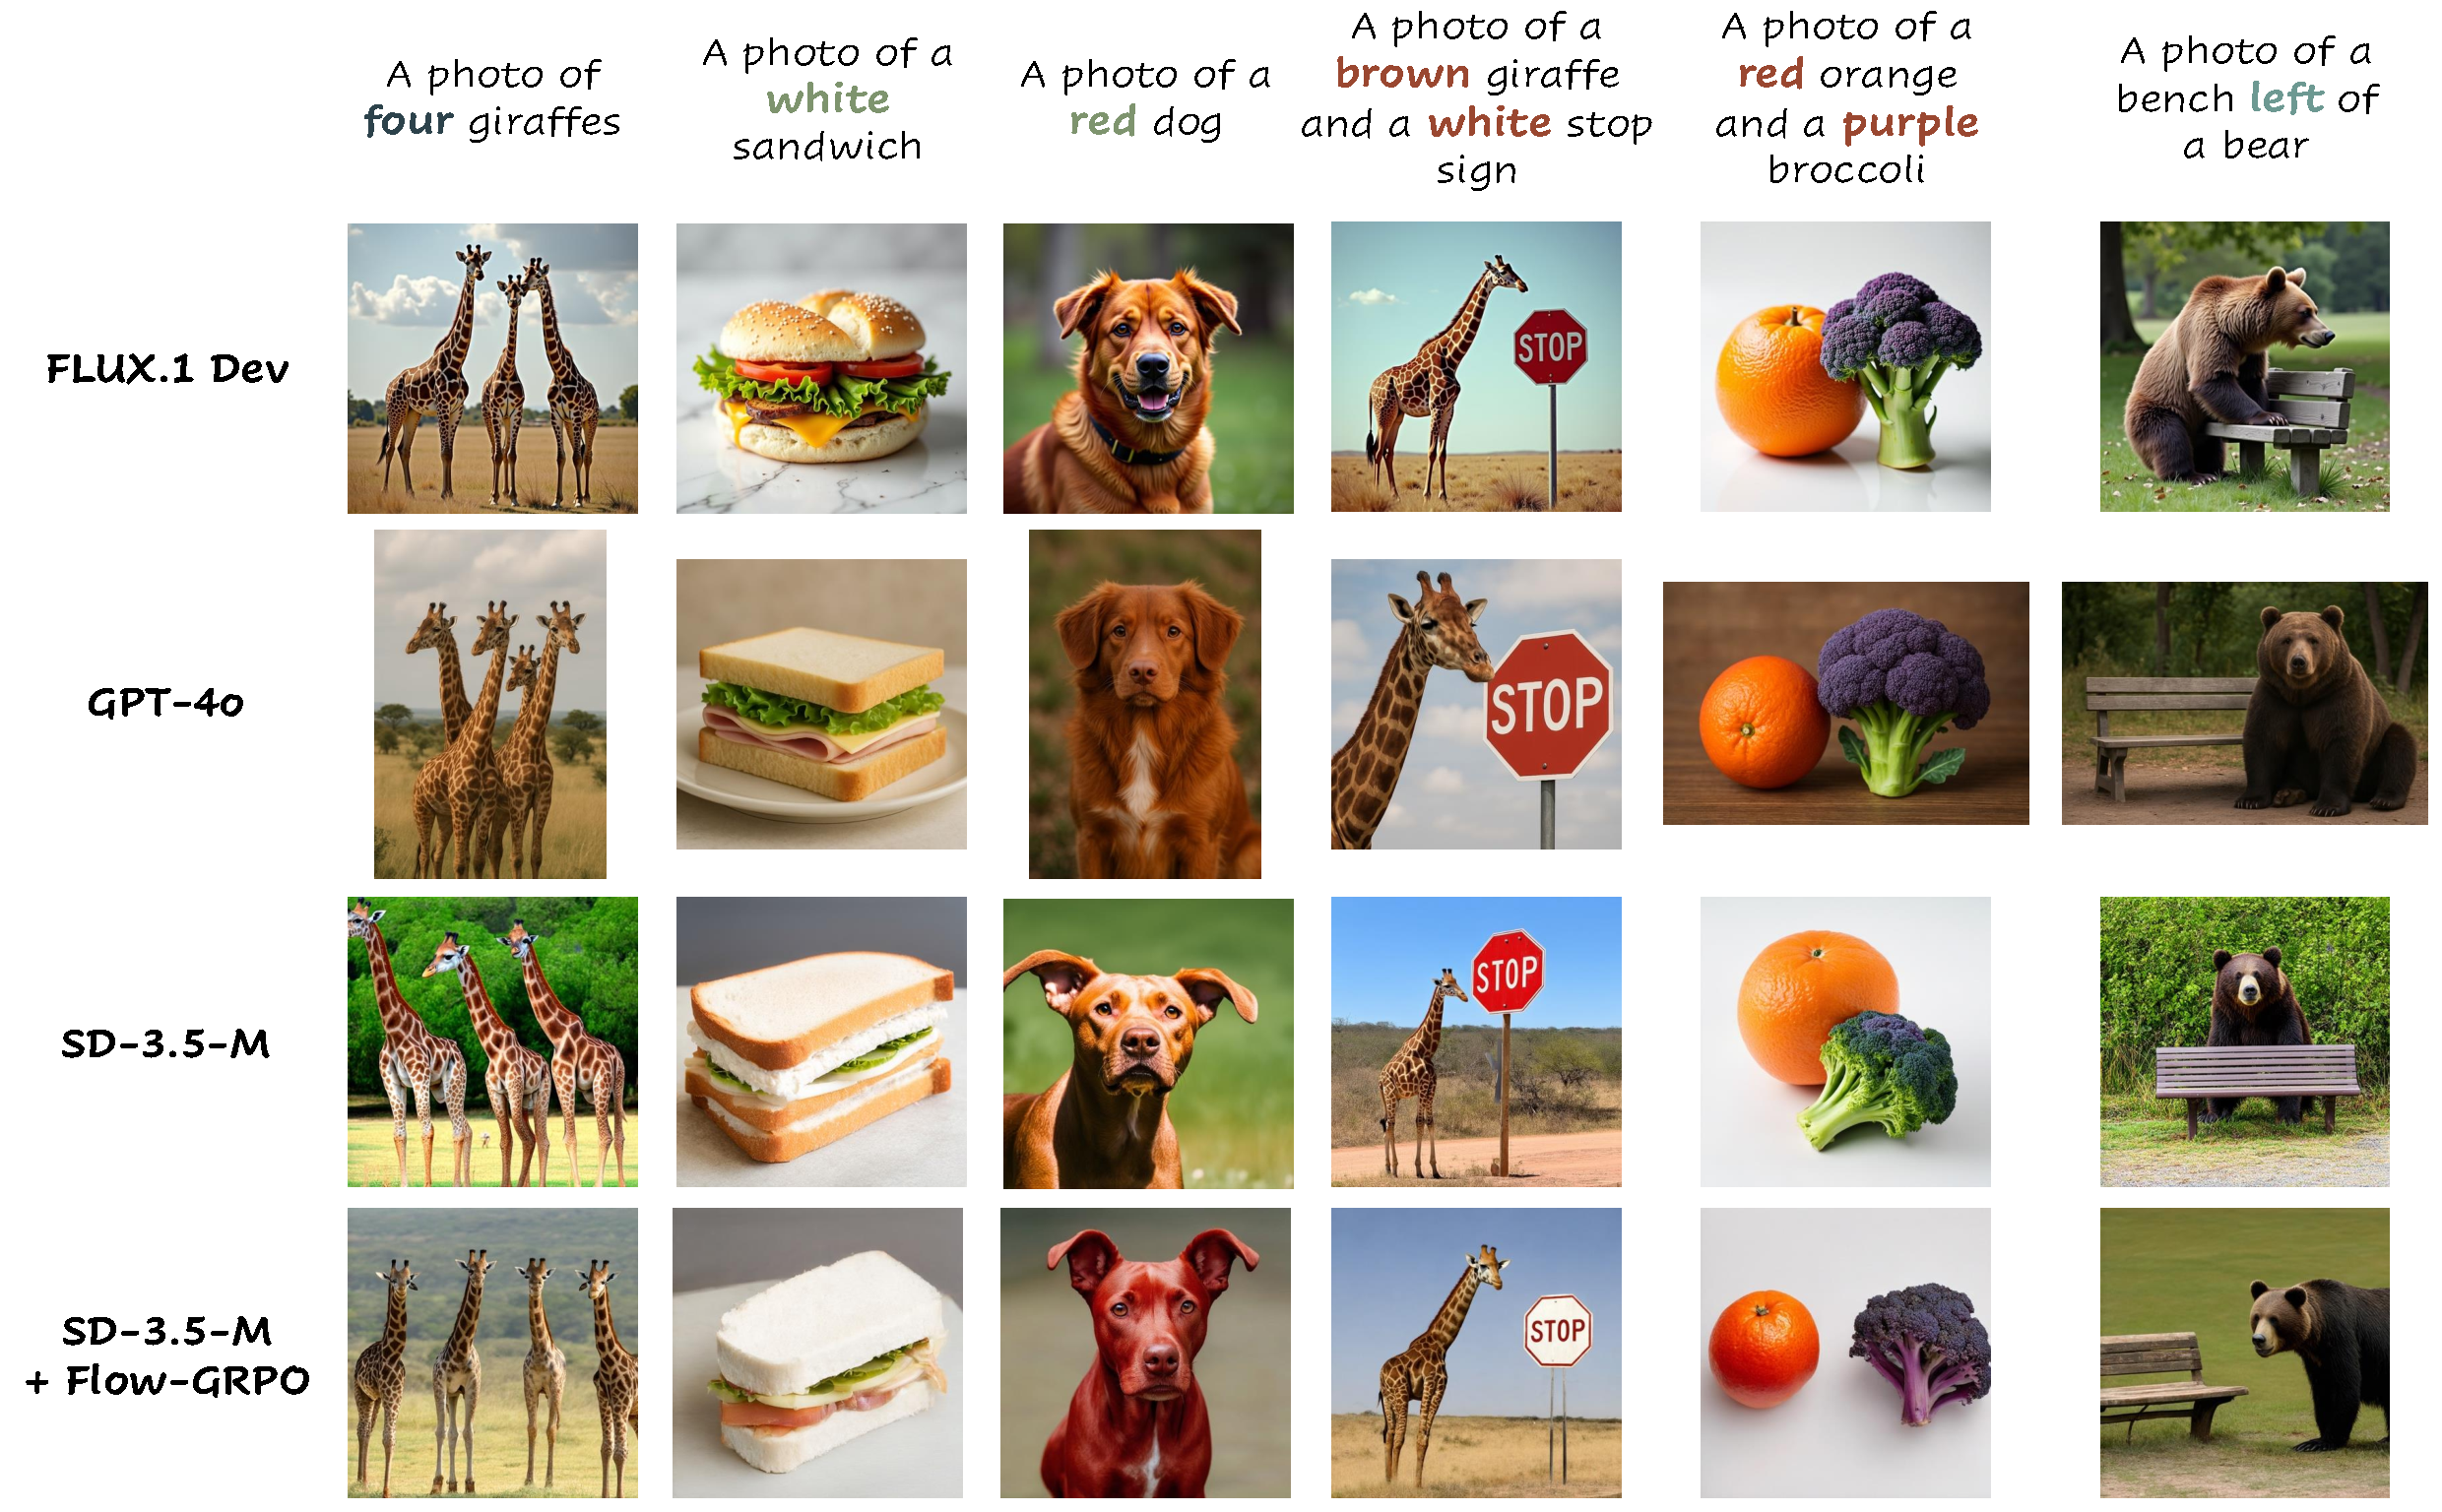
\includegraphics[width=\textwidth]{src/experiments/result_geneval.pdf}
\caption{\textbf{Qualitative Comparison on the GenEval Benchmark.} Our approach demonstrates superior performance in 
\textbf{\textcolor{pltcount}{Counting}}, 
\textbf{\textcolor{pltcolor}{Colors}}, 
\textbf{\textcolor{pltattr}{Attribute Binding},
and \textbf{\textcolor{pltpos}{Position}}}.
}
\vspace{-2mm}
\label{fig:result_geneval}
\end{figure}


\begin{table*}[t]
    \centering
    \renewcommand{\arraystretch}{1.1}
    \caption{\textbf{Performance on Compositional Image Generation, Visual Text Rendering, and Human Preference} benchmarks, evaluated by task performance on test prompts, and by image quality and preference scores on DrawBench prompts. ImgRwd: ImageReward; UniRwd: UnifiedReward.}
    \resizebox{\linewidth}{!}{
        \begin{tabular}{lcccccccc}
            \toprule
            \multirow{2}{*}{\textbf{Model}} & \multicolumn{3}{c}{\textbf{Task Metric}} & \multicolumn{2}{c}{\textbf{Image Quality}} & \multicolumn{3}{c}{\textbf{Preference Score}}    \\ \cmidrule(lr){2-4} \cmidrule(lr){5-6} \cmidrule(l){7-9} 
                                   & \textbf{GenEval}  & \textbf{OCR Acc.}  & \textbf{PickScore} & \textbf{Aesthetic}          & \textbf{DeQA}         & \textbf{ImgRwd} & \textbf{PickScore} & \textbf{UniRwd} \\ \midrule
            SD3.5-M & 0.63 & 0.59 & 21.72 & 5.39 & 4.07 & 0.87 & 22.34 & 3.33 \\
            \midrule
            % \addlinespace[3pt]
            % \rowcolor{gray!15}
            \multicolumn{9}{c}{\textit{Compositional Image Generation}} \\
            \midrule
            % \rowcolor{gray!05}
            Flow-GRPO (w/o KL) & 0.95 & — & — & 4.93 & 2.77 & 0.44 & 21.16 & 2.94 \\
            % \rowcolor{gray!05}
            \rowcolor{gray!20} Flow-GRPO (w/ KL)  & 0.95 & — & — & 5.25 & 4.01 & 1.03 & 22.37 & 3.51 \\

            \midrule
            % \addlinespace[3pt]
            % \rowcolor{gray!15}
            \multicolumn{9}{c}{\textit{Visual Text Rendering}} \\
            \midrule
            Flow-GRPO (w/o KL) & — & 0.93 & — & 5.13 & 3.66 & 0.58 & 21.79 & 3.15 \\
            \rowcolor{gray!20} Flow-GRPO (w/ KL)  & — & 0.92 & — & 5.32 & 4.06 & 0.95 & 22.44 & 3.42 \\
            
            \midrule
            % \rowcolor{gray!15}
            \multicolumn{9}{c}{\textit{Human Preference Alignment}} \\
            \midrule
            % \rowcolor{gray!05}
            Flow-GRPO (w/o KL) & — & — & 23.41 & 6.15 & 4.16 & 1.24 & 23.56 & 3.57 \\
            % \rowcolor{gray!05}
            \rowcolor{gray!20} Flow-GRPO (w/ KL)  & — & — & 23.31 & 5.92 & 4.22 & 1.28 & 23.53 & 3.66 \\
            \bottomrule
            \end{tabular}
}
\vspace{-2mm}
\label{tab:all_task}
\end{table*}


% \begin{figure}[htbp]
% \centering
% \includegraphics[width=0.9\textwidth]{src/experiments/compare_curve3.pdf}
% \caption{Comparison of Flow-GRPO and Other Alignment Methods on the Compositional Image Generation task. \todo
% }
% \label{app:fig:compare_curva_geneval}
% \end{figure}

\begin{figure}[htbp]
  \centering
  \begin{minipage}[t]{0.49\textwidth}
    \centering
    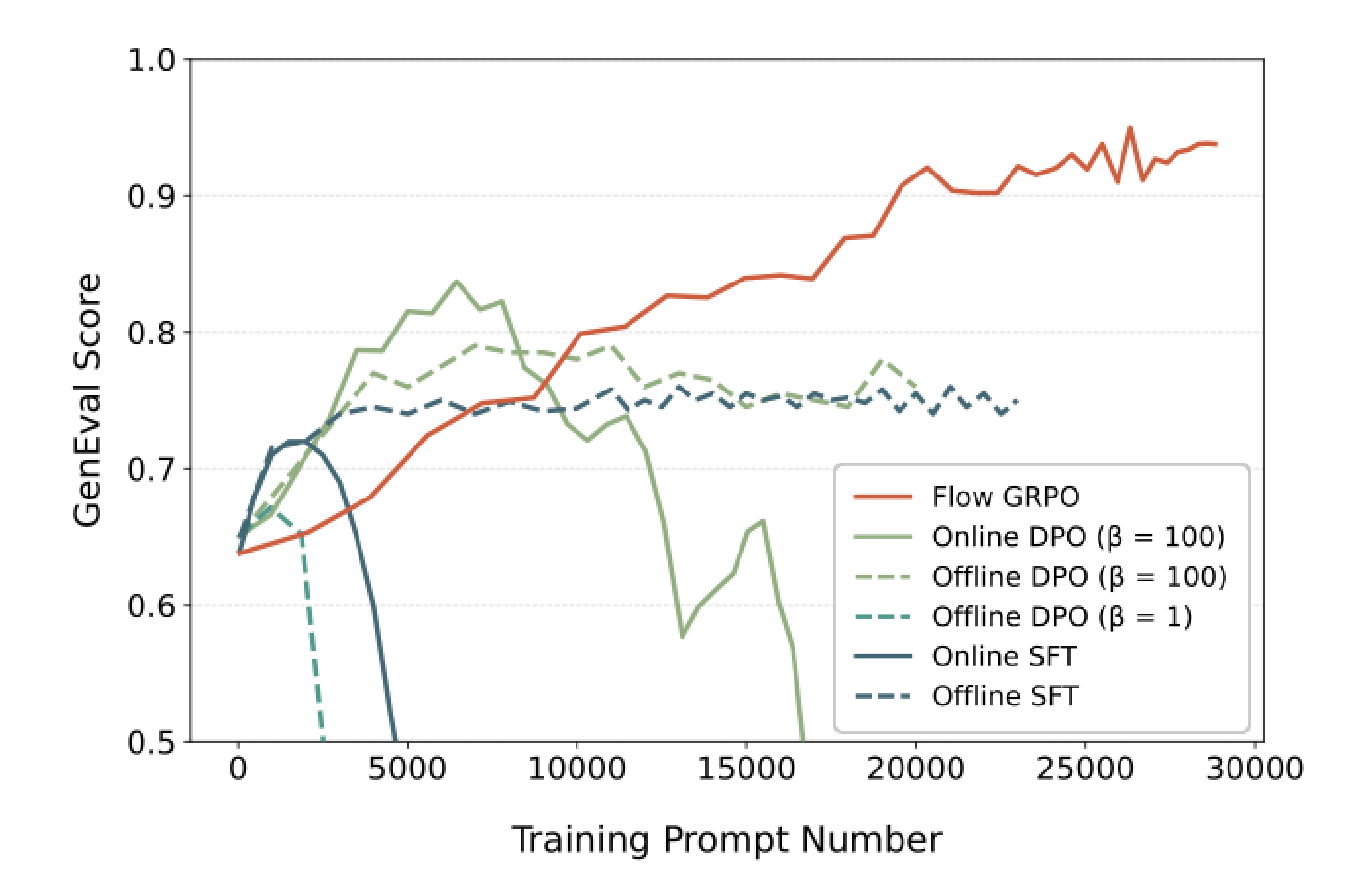
\includegraphics[width=\linewidth]{src/experiments/compare_curve_3.pdf}
    \vspace{-1.5em}
    \caption{
    Comparison with Other Alignment Methods on the Compositional Generation Task.
    % Comparison with Other Alignment Methods on the GenEval Task.
    }
    \label{app:fig:compare_curva_geneval}
  \end{minipage}
  \hfill
  \begin{minipage}[t]{0.47\textwidth}
    \centering
    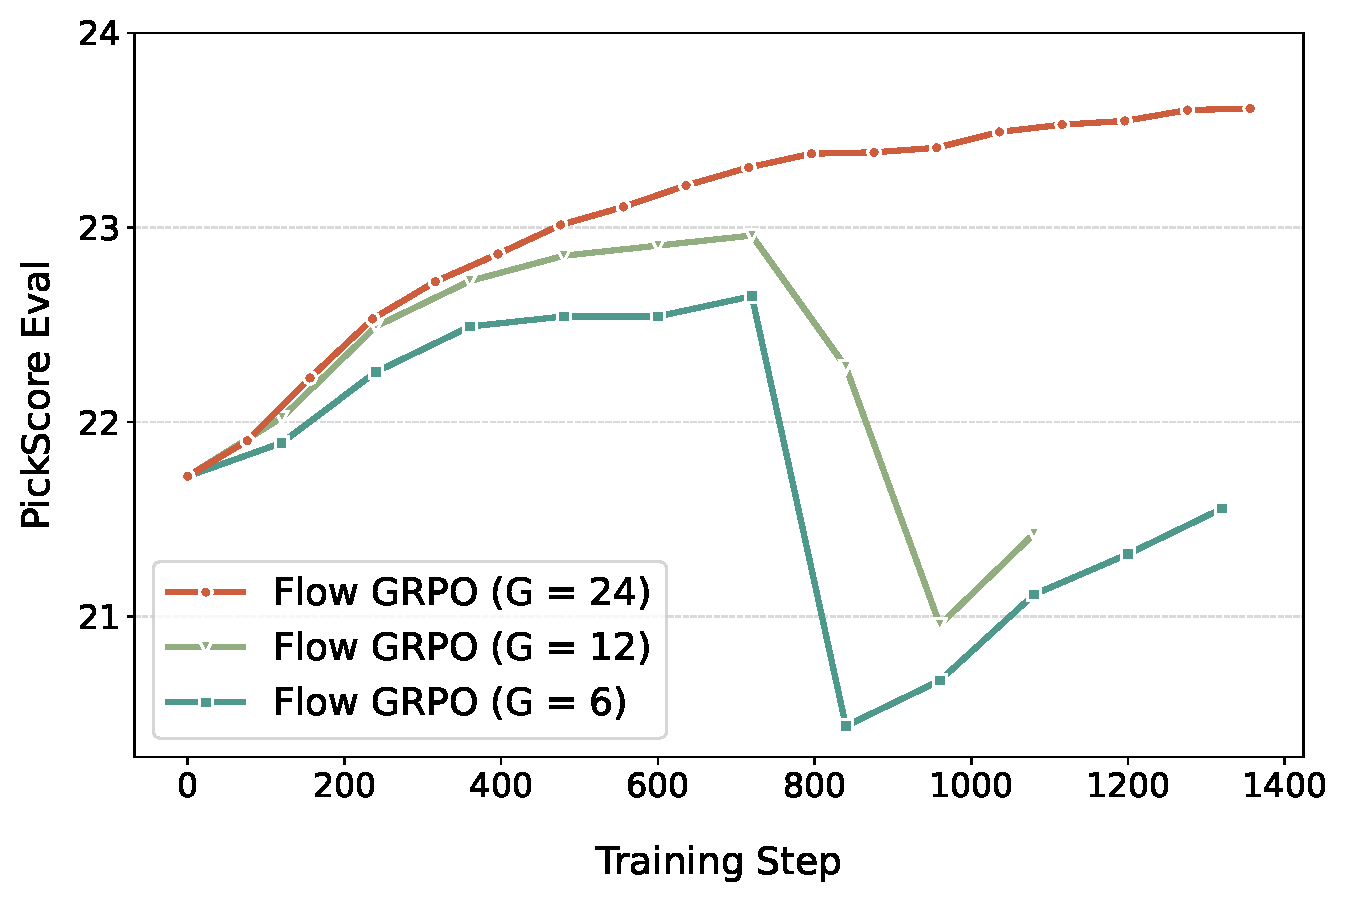
\includegraphics[width=\linewidth]{src/experiments/camera_ready_add/camera_ready_group.pdf}
    \vspace{-1.5em}
    \caption{Ablation Studies on Different Group Size $G$. Higher group size performs better.}
    \label{fig:abltion_groupsize}
  \end{minipage}
\end{figure}
% \paragraph{Results.} 

% **Experiments**  

\subsection{Main Results}  
Figure~\ref{fig:teaser} and Table~\ref{tab:geneval} show Flow-GRPO's GenEval performance steadily improving during training, ultimately outperforming GPT-4o. This occurs while maintaining both image quality metrics and preference scores on DrawBench, a benchmark with diverse and comprehensive prompts for evaluating general model capabilities. Figure~\ref{fig:result_geneval} offers qualitative comparisons.
Beyond Compositional Image Generation, Table~\ref{tab:all_task} details evaluations on Visual Text Rendering and Human Preference tasks. Flow-GRPO improved text rendering ability, again without decreasing image quality metrics and preference scores on DrawBench. 
See Figures~\ref{app:fig:add_qualitative_result_geneval}, \ref{app:fig:add_qualitative_result_ocr} \& \ref{app:fig:add_qualitative_result_pickscore} in Appendix~\ref{app:subsec:qualitative_results} for related qualitative examples.
For the Human Preference task, image quality did not decrease without KL regularization. However, we found that omitting KL caused a collapse in visual diversity, a form of reward hacking discussed further in Section~\ref{sec:subsec:reward_hacking}.
These results demonstrate that Flow-GRPO boosts desired capabilities while causing very little degradation to image quality or visual diversity.

% We also compare Flow-GRPO with other alignment methods, including supervised fine-tuning, reward weighted regression~\cite{videoalign, awr}, Flow-DPO~\cite{videoalign}, and their online variants. Flow-GRPO outperforms all of them by a large margin. See Appendix~\ref{app:subsec:baselines} for details.
\paragraph{Flow-GRPO vs. Other Alignment Methods.}
We compare Flow-GRPO with several alignment methods: supervised fine-tuning (SFT), Flow-DPO~\cite{videoalign,wallace2024diffusion}, and their online variants. Flow-GRPO consistently outperforms all baselines by a significant margin.
At each step, we generate a group of images using the same group size as in Flow-GRPO. The only difference lies in the update rule:
\begin{itemize}
\setlength{\itemindent}{-2em}
\item \textbf{SFT}: Select the highest-reward image in each group and fine-tune on it.
\item \textbf{Flow-DPO}: Use the highest-reward image in each group as the chosen sample and the lowest as the rejected, then apply the DPO loss.
\end{itemize}

Offline variants use a fixed pretrained model for data collection, while online variants update their data collection models every 40 steps. As shown in Figure~\ref{app:fig:compare_curva_geneval}, Flow-GRPO outperforms all baselines. Online DPO also surpasses its offline counterpart, consistent with~\cite{skyreels_v2}. For the second-best online DPO, a hyperparameter search on its key parameter $\beta$ revealed that smaller values are not always optimal; excessively small $\beta$ values can cause training collapse. Appendix~\ref{app:sec:extened-exp-results} presents more comprehensive comparisons covering additional methods and tasks.

% \begin{table}[ht]
% \centering
% \begin{tabular}{l|lccccccc}
% \toprule
% % \multirow{2}{*}
% {\textbf{Type}} & {\textbf{Method}} &  \textbf{Single Obj.} & \textbf{Two Obj.} & \textbf{Counting} & \textbf{Colors} & \textbf{Position} & \textbf{Color Attr.} & \textbf{Overall} \\ 
% \midrule

% \multirow{6}{*}{\textbf{Diffusion Only}} 
% & SDXL [88] & 98 & 74 & 39 & 85 & 15 & 23 & 55 \\ 
% & FLUX.1-dev [57] & 98 & 79 & 73 & 77 & 22 & 45 & 66 \\ 
% & DALL-E 3 [100] & 96 & 87 & 47 & 83 & 43 & 45 & 67 \\ 
% & SD3-Medium [24] & 99 & 94 & 72 & 89 & 33 & 60 & 74 \\ 
% & CogView4-6B [3] & 99 & 86 & 66 & 79 & 48 & 58 & 73 \\ 
% \midrule

% \multirow{5}{*}{\textbf{Hybrid Model}} 
% & SEED-X [29] & 97 & 58 & 26 & 80 & 19 & 14 & 49 \\ 
% & Transfusion [133] & - & - & - & - & - & - & 63 \\
% & D-DiT [64] & 97 & 80 & 54 & 76 & 32 & 50 & 65 \\ 
% & Show-o [124] & 98 & 80 & 66 & 84 & 31 & 50 & 68 \\ 
% & GPT-4ot [81] & 99 & 92 & 85 & 91 & 75 & 66 & 85 \\
% % \hline
% \bottomrule
% \end{tabular}
% \caption{Performance comparison of different methods across metrics.}
% \label{tab:comparison}
% \end{table}

% \begin{table}[ht]
% \centering
% \caption{Performance comparison of different methods across metrics. ``Single Obj.'', ``Two Obj.'', ``Pos.'' and ``Attr. binding'' denote ``Single Object'', ``Two Object'', ``Position'' and ``Attribute binding'', respectively.}

% \begin{tabular}{l|ccccccc}
% \toprule
% % \multirow{2}{*}
%  {\textbf{Method}} &  \textbf{Single Obj.} & \textbf{Two Obj.} & \textbf{Counting} & \textbf{Colors} & \textbf{Pos.} & \textbf{Attr. binding} & \textbf{Overall} \\ 
% \midrule
% \multicolumn{8}{c}{\textit{Diffusion Only}} \\
% \midrule

% SDXL & 98 & 74 & 39 & 85 & 15 & 23 & 55 \\ 
% FLUX.1-dev  & 98 & 79 & 73 & 77 & 22 & 45 & 66 \\ 
% DALL-E3 & 96 & 87 & 47 & 83 & 43 & 45 & 67 \\ 
% SD3-Medium & 99 & 94 & 72 & 89 & 33 & 60 & 74 \\ 
% CogView4-6B & 99 & 86 & 66 & 79 & 48 & 58 & 73 \\ 
% \midrule
% \multicolumn{8}{c}{\textit{Hybrid Model}} \\
% \midrule
% % \multirow{5}{*}{\textbf{Hybrid Model}} 
% SEED-X & 97 & 58 & 26 & 80 & 19 & 14 & 49 \\ 
% Transfusion & - & - & - & - & - & - & 63 \\
% D-DiT& 97 & 80 & 54 & 76 & 32 & 50 & 65 \\ 
% Show-o & 98 & 80 & 66 & 84 & 31 & 50 & 68 \\ 
% GPT-4o & 99 & 92 & 85 & 91 & 75 & 66 & 85 \\
% % \hline
% \bottomrule
% \end{tabular}
% \label{tab:comparison}
% \end{table}

% **Implementation Details:** All experiments use Stable Diffusion 3 (SD3) with LoRA fine-tuning (rank=32) and timestep fraction scheduling. Training runs on 24–32 GPUs with KL regularization (β=0.004–0.04) unless specified.  


% \begin{figure}[t]
% \centering
% 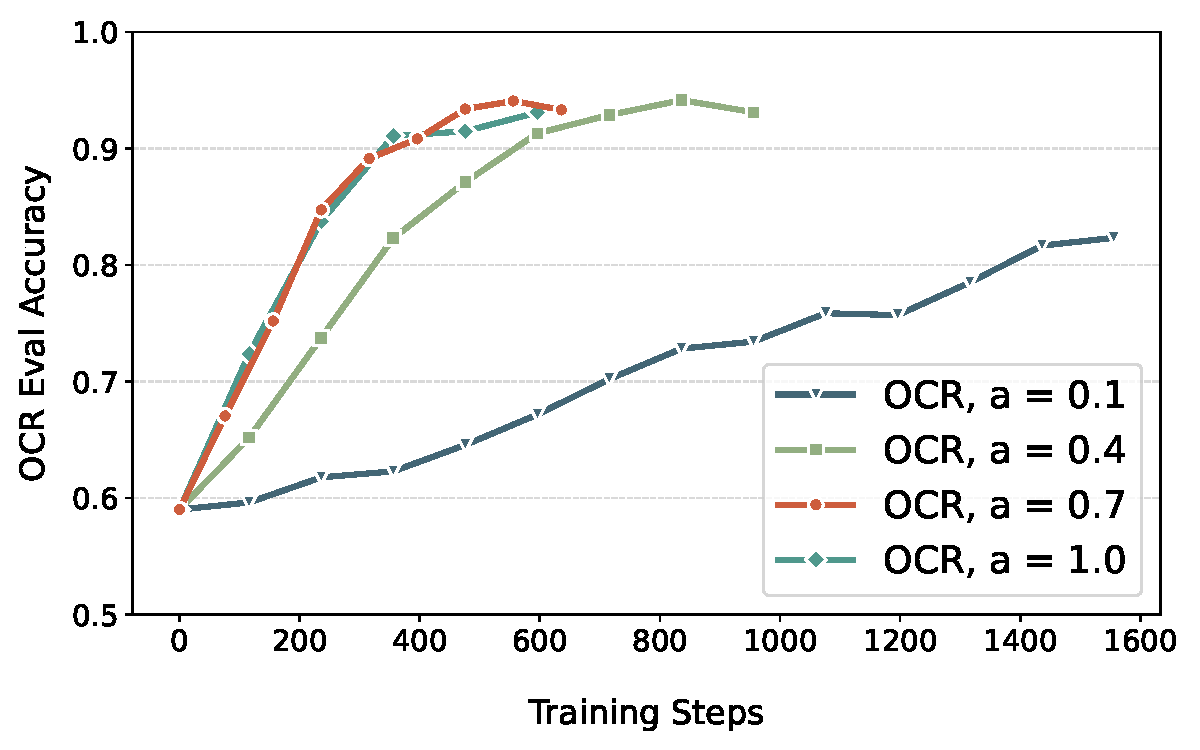
\includegraphics[width=0.5\textwidth]{src/experiments/ablation_noise/exp1_ocr_ablation_noise.pdf}
% \caption{Increasing the noise level $a$ boosts exploration and speeds up training.
% }
% \label{fig:exp1_ocr_ablation_noise}
% \end{figure}

% \begin{figure}[htbp]
%   \centering
%   \begin{minipage}[t]{0.48\textwidth}
%     \centering
%     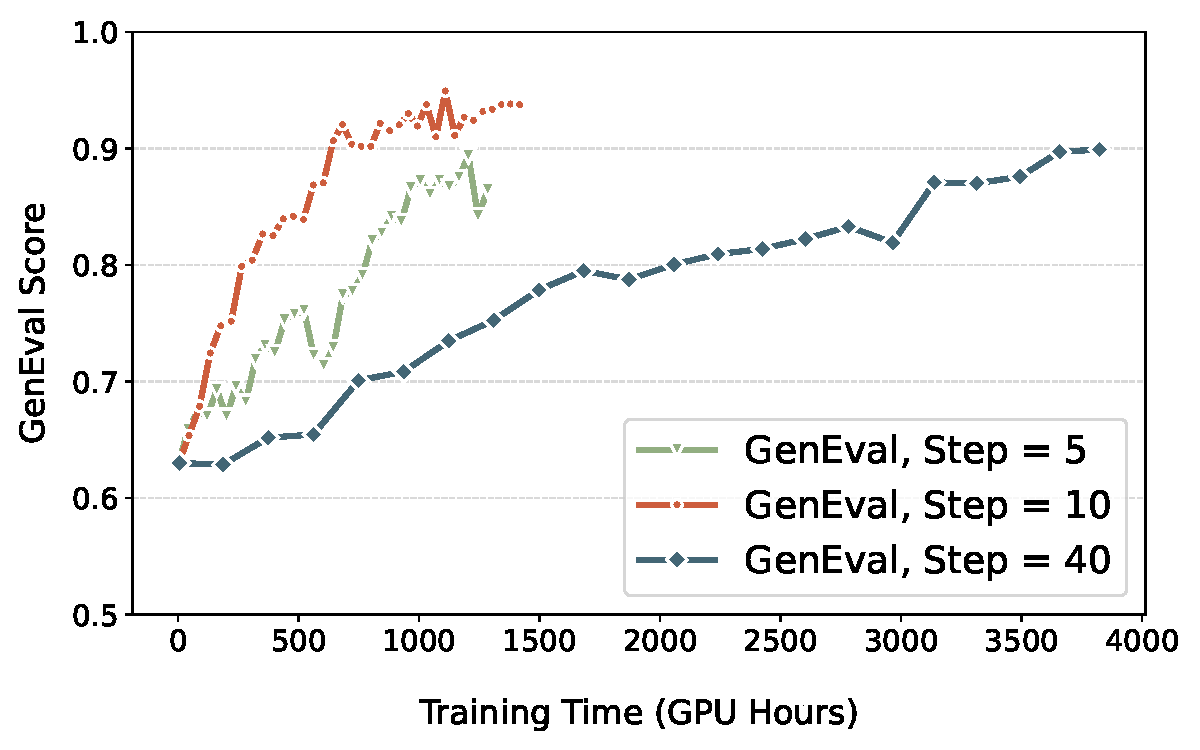
\includegraphics[width=\linewidth]{src/experiments/ablation_step/exp2_geneval_ablation_step.pdf}
%     \vspace{-1.5em}
%     \caption*{\footnotesize (a). Experiments on GenEval}
%   \end{minipage}
%   \hfill
%   \begin{minipage}[t]{0.48\textwidth}
%     \centering
%     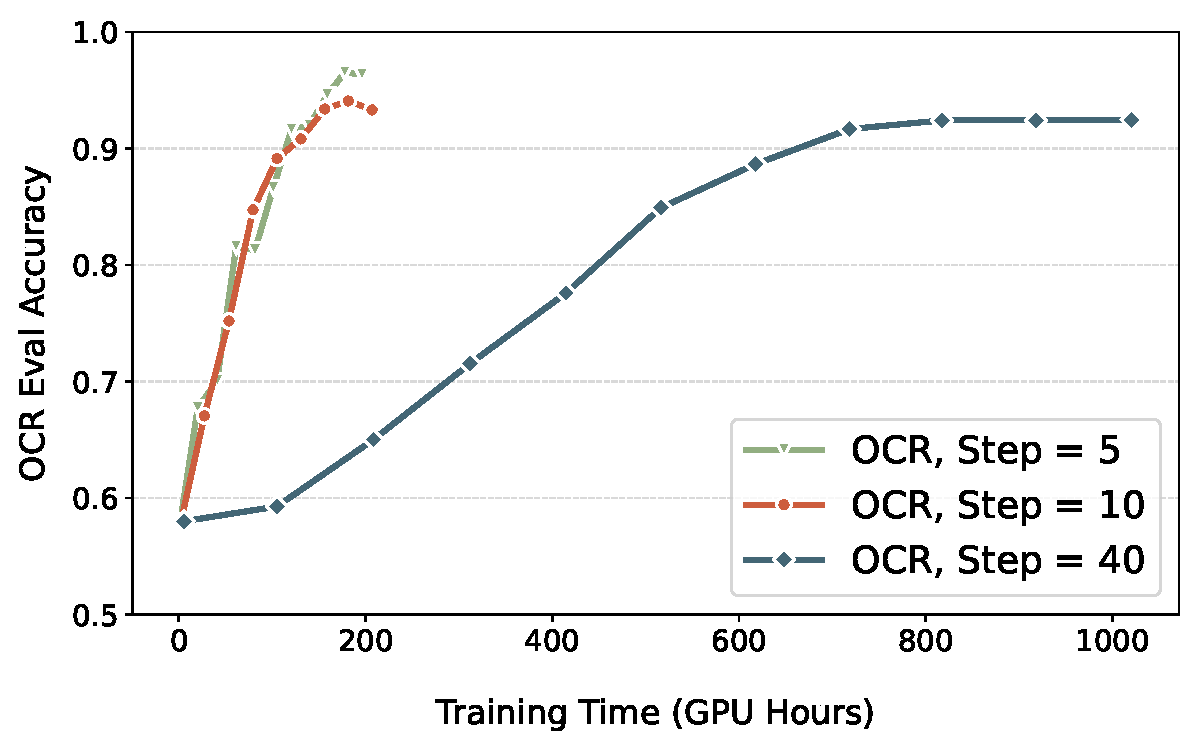
\includegraphics[width=\linewidth]{src/experiments/ablation_step/exp2_ocr_ablation_step.pdf}
%     \vspace{-1.5em}
%     \caption*{\footnotesize (b).  Experiments on OCR}
%   \end{minipage}
%   \vspace{1.5em}

%   \begin{minipage}[t]{0.48\textwidth}
%     \centering
%     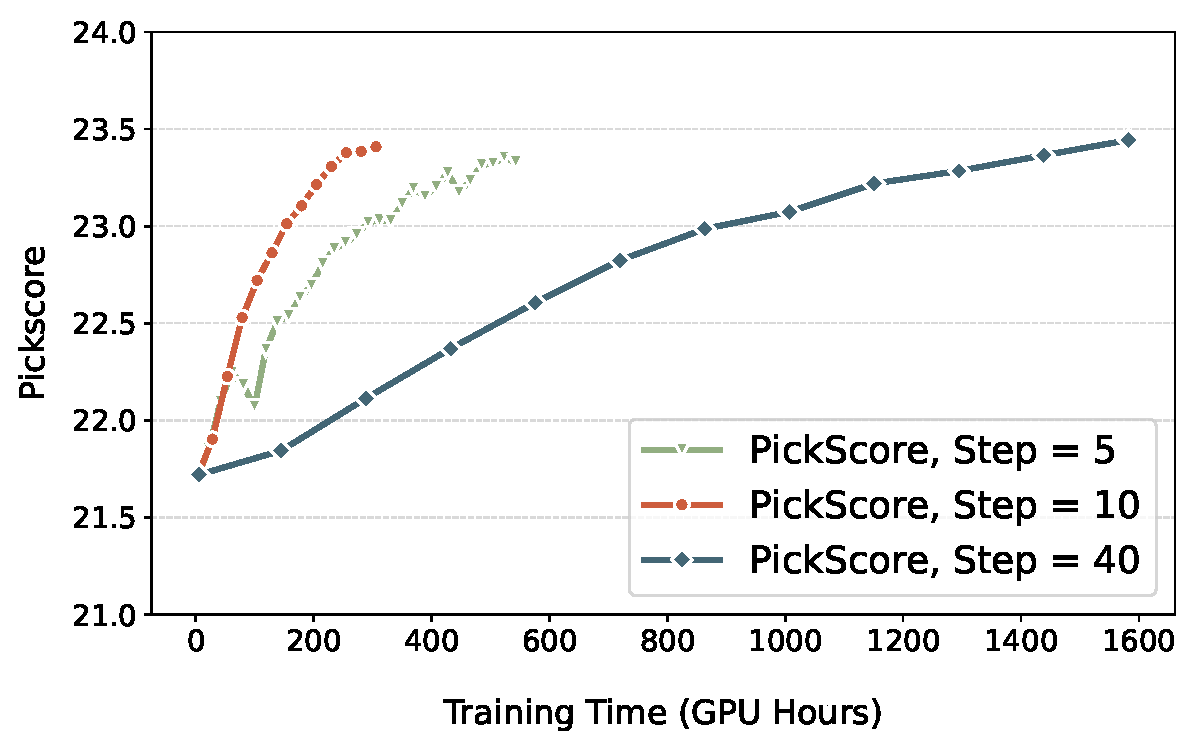
\includegraphics[width=\linewidth]{src/experiments/ablation_step/exp2_pickscore_ablation_step.pdf}
%     \vspace{-1.5em}
%     \caption*{\footnotesize (c). Experiments on PickScore}
%   \end{minipage}

%   \caption{To be added}
%   \label{fig:exp2_ablation_step}
% \end{figure}


% \begin{figure}[htbp]
%   \centering
%   \begin{minipage}[t]{0.48\textwidth}
%     \centering
%     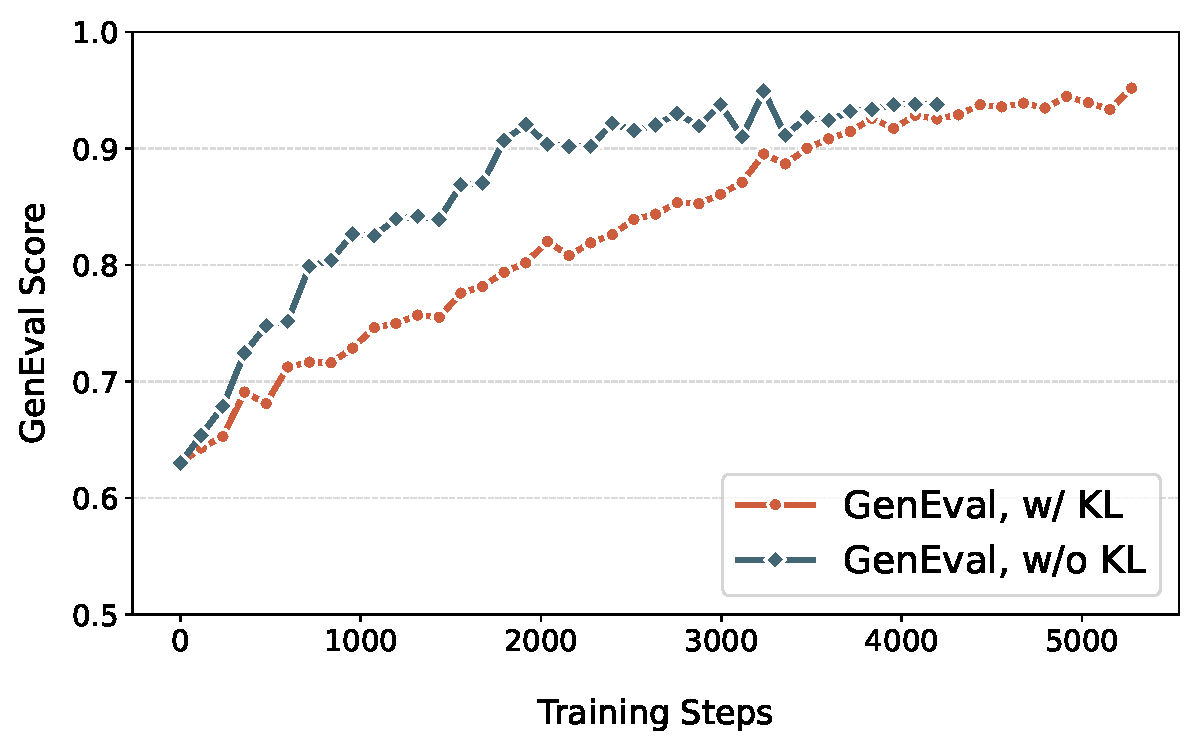
\includegraphics[width=\linewidth]{src/experiments/ablation_kl/exp3_geneval_ablation_kl.pdf}
%     \vspace{-1.5em}
%     \caption*{\footnotesize (a). Experiments on GenEval}
%   \end{minipage}
%   \hfill
%   \begin{minipage}[t]{0.48\textwidth}
%     \centering
%     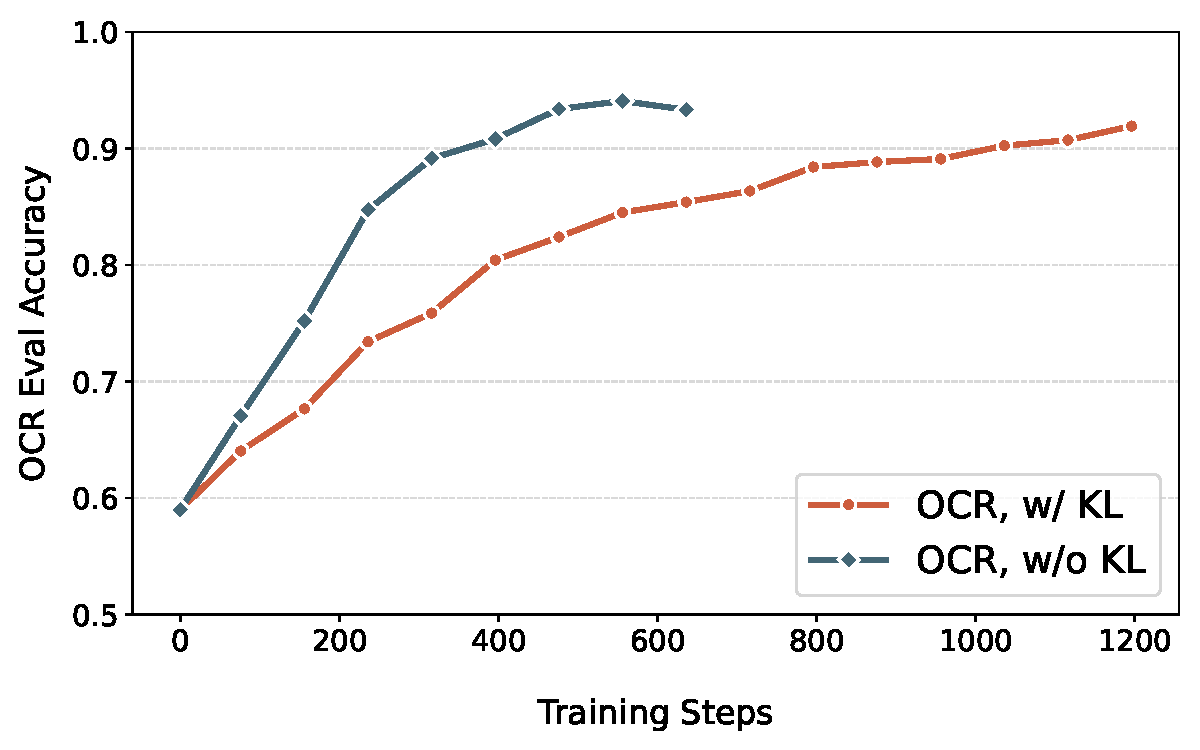
\includegraphics[width=\linewidth]{src/experiments/ablation_kl/exp3_ocr_ablation_kl.pdf}
%     \vspace{-1.5em}
%     \caption*{\footnotesize (b).  Experiments on OCR}
%   \end{minipage}
%   \vspace{1.5em}

%   \begin{minipage}[t]{0.48\textwidth}
%     \centering
%     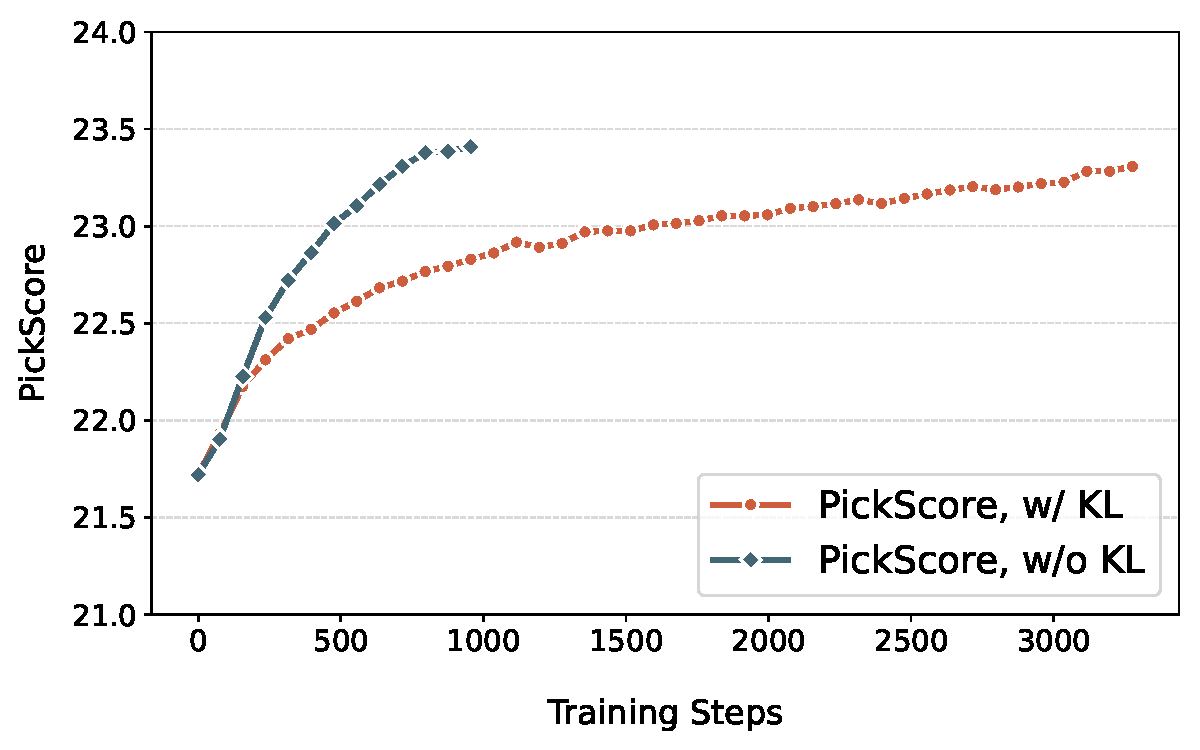
\includegraphics[width=\linewidth]{src/experiments/ablation_kl/exp3_pickscore_ablation_kl.pdf}
%     \vspace{-1.5em}
%     \caption*{\footnotesize (c). Experiments on PickScore}
%   \end{minipage}

%   \caption{To be added}
%   \label{fig:exp3_ablation_kl}
% \end{figure}

% \begin{figure}[htbp]
%   \centering
%   \begin{minipage}[t]{0.48\textwidth}
%     \centering
%     \includegraphics[width=\linewidth]{src/experiments/ablation_both/exp23_geneval_ablation.pdf}
%     \vspace{-1.5em}
%     \caption*{\footnotesize (a). Experiments on GenEval}
%   \end{minipage}
%   \hfill
%   \begin{minipage}[t]{0.48\textwidth}
%     \centering
%     \includegraphics[width=\linewidth]{src/experiments/ablation_both/exp23_ocr_ablation.pdf}
%     \vspace{-1.5em}
%     \caption*{\footnotesize (b).  Experiments on OCR}
%   \end{minipage}
%   \vspace{1.5em}

%   \begin{minipage}[t]{0.48\textwidth}
%     \centering
%     \includegraphics[width=\linewidth]{src/experiments/ablation_both/exp23_pickscore_ablation.pdf}
%     \vspace{-1.5em}
%     \caption*{\footnotesize (c). Experiments on PickScore}
%   \end{minipage}

%   \caption{To be added}
%   \label{fig:exp23_ablation_}
% \end{figure}




% \subsection{Ablation Study}
% \paragraph{}

\subsection{Analysis}
This section presents several analyses to better understand the behavior and robustness of Flow-GRPO. We examine issues such as reward hacking, the impact of denoising reduction and noise levels, the effect of group size, and the model’s generalization ability. We provide additional analyses in the Appendix~\ref{app:sec:extened-exp-results}.

\paragraph{Reward Hacking.}\label{sec:subsec:reward_hacking}
We use KL regularization to mitigate reward hacking by tuning the KL coefficient to keep the divergence small and nearly 
 constant during training, keeping the model close to its pretrained weights. This allows task-specific reward optimization without harming overall performance.
As shown in Table~\ref{tab:all_task}, removing the KL constraint for Compositional Image Generation and Visual Text Rendering significantly reduces image quality and preference scores on DrawBench. In contrast, a properly tuned KL preserves quality while achieving similar gains on task-specific metrics.
In the Human Preference Alignment task, removing KL does not affect image quality, likely due to overlap between PickScore and evaluation metrics, but causes a collapse in visual diversity. Outputs converge to a single style, with different seeds producing nearly identical results. KL regularization prevents this collapse and maintains diversity.
See Figure~\ref{app:fig:exp3_ablation_kl} in Appendix~\ref{app:subsec:training_curve_kl} for training curves and Figure~\ref{fig:quality_divesity_example} for more examples.

\definecolor{pltcount}{HTML}{2C424B}
\definecolor{pltcolor}{HTML}{7E946E}
\definecolor{pltpos}{HTML}{6D9992}
\definecolor{pltattr}{HTML}{9A4730}
\begin{figure}[t]
\centering
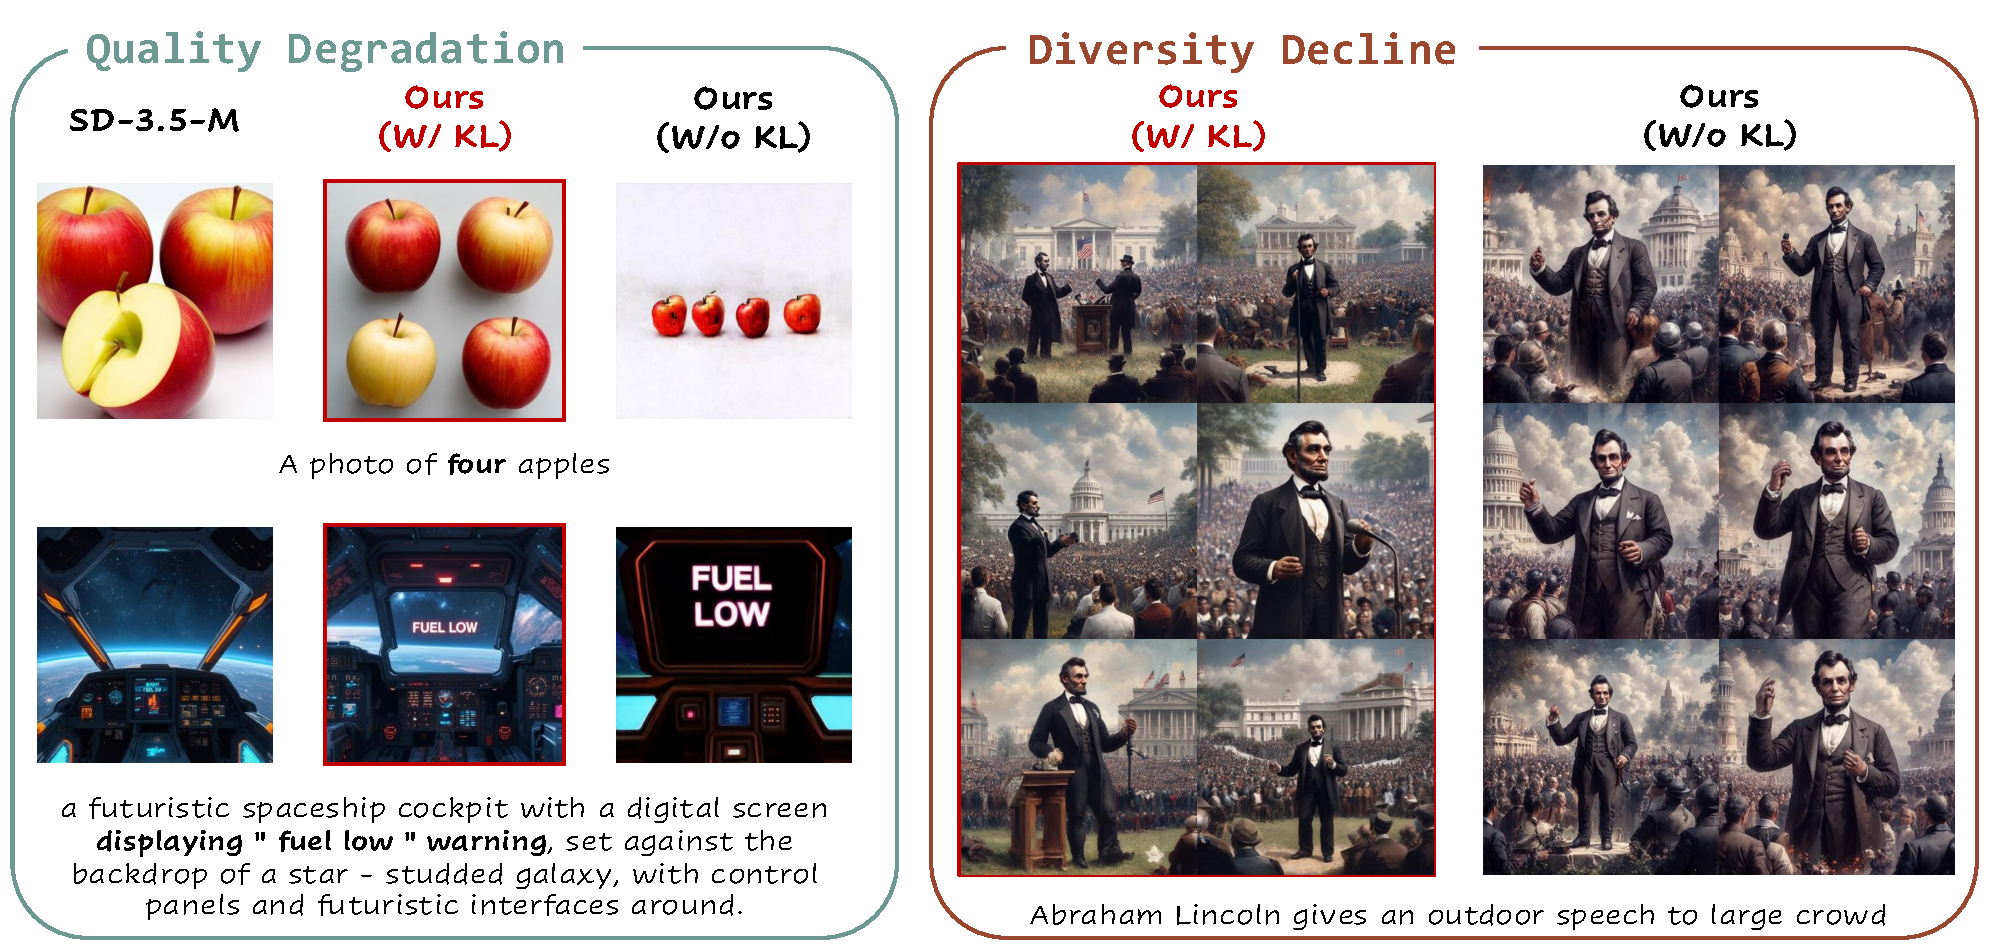
\includegraphics[width=\textwidth]{src/experiments/ablation_kl.pdf}
\caption{\textbf{Effect of KL Regularization.} The KL penalty effectively suppresses reward hacking, preventing
\textbf{\textcolor{pltpos}{Quality Degradation}} (for GenEval and OCR) and  
\textbf{\textcolor{pltattr}{Diversity Decline}} (for PickScore).
}
\vspace{-3mm}
\label{fig:quality_divesity_example}
\end{figure}

\paragraph{Effect of Denoising Reduction.}
Figure~\ref{fig:exp_ablation} (a) highlights Denoising Reduction's significant impact on accelerating training. To explore how different timesteps affect optimization, these experiments are conducted without the KL constraint. Reducing data collection timesteps from $40$ to $10$ achieves over a $4\times$ speedup across all three tasks, without impacting final reward. Further reducing to $5$ does not consistently improve speed and sometimes slows training, so we choose $10$ timesteps for later experiments. For the other two tasks, learning curves of reward versus training time are presented in Figure~\ref{app:fig:exp2_ablation_step} in the Appendix~\ref{app:subsec:noising_reduction}.



\paragraph{Effect of Noise Level.}\label{sec:exp:noise_scheduler}
% 提高SDE中的$\sigma_t$可以给生成的图片带来更多的多样性，从而提升exploration，这对rl训练至关重要。As in Eq.~\ref{eq:update_rule}, we control the exploration by the Noise level 系数$a$.
% We conduct ablations to study how the noise level $a$ influences performance. Figure~\ref{} presents results for different values of $a$. Small noise levels (e.g., $a = 0.1$) limit exploration and lead to slow reward improvement. Increasing $a$ (up to 0.7) enhances exploration and accelerates reward gains. However, beyond a certain point, further increasing the noise (e.g., $a = 0.7\rightarrow1.0$) brings no additional benefit as the exploration space is already sufficient for learning. We also observe that overly large noise levels severely degrade image quality, causing the reward to remain at zero and preventing effective training. We recommend using the highest noise level that does not significantly harm image quality.
Higher $\sigma_t$ in the SDE boosts image diversity and exploration, vital for RL training. We control this exploration with a noise level $a$ (Eq.~\ref{eq:update_rule}).
Figure~\ref{fig:exp_ablation} (b) shows the impact of $a$ on performance. A small $a$ (e.g., 0.1) limits exploration and slows reward improvement. Increasing $a$ (up to 0.7) boosts exploration and speeds up reward gains. Beyond this point (e.g., from 0.7 to 1.0), further increases provide no additional benefit, as exploration is already sufficient. We also observe that injecting too much noise by further increasing $a$ degrades image quality, resulting in zero reward and failed training. 

\begin{figure}[htbp]
  \centering
  \begin{minipage}[t]{0.48\textwidth}
    \centering
    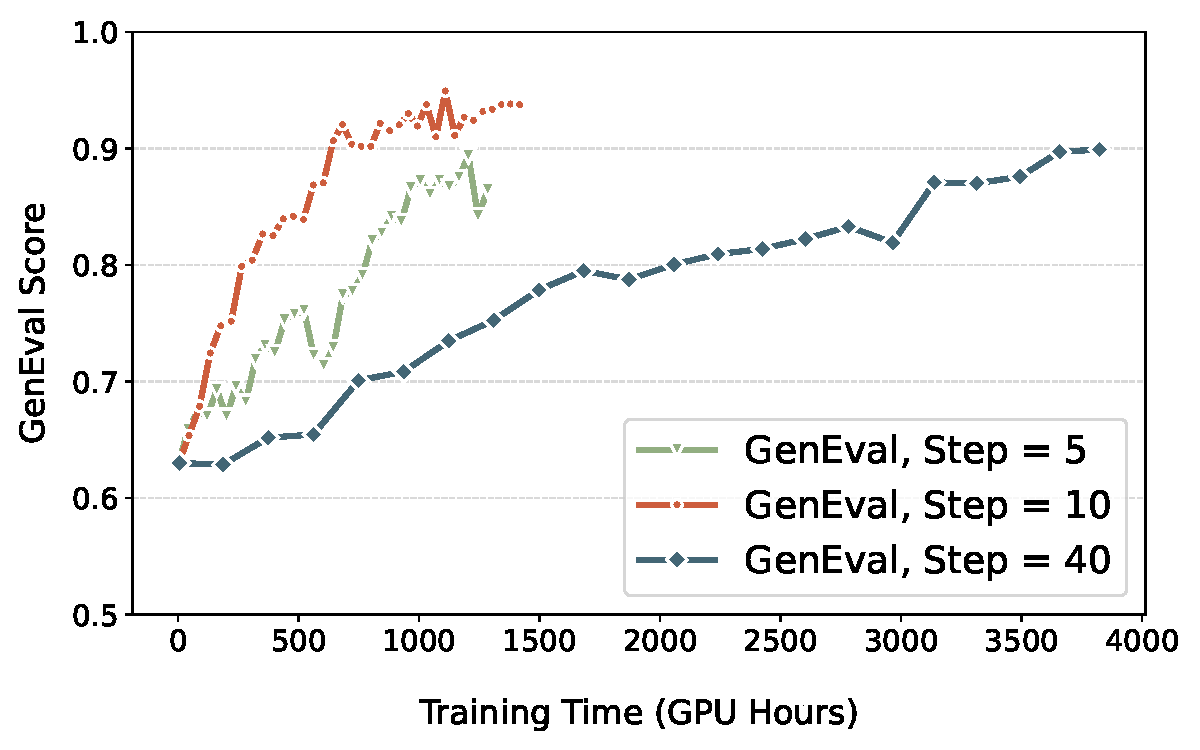
\includegraphics[width=\linewidth]{src/experiments/ablation_step/exp2_geneval_ablation_step.pdf}
    \vspace{-1.5em}
    \caption*{\footnotesize (a). Effect of Denoising Reduction on GenEval}
  \end{minipage}
  \hfill
  \begin{minipage}[t]{0.48\textwidth}
    \centering
    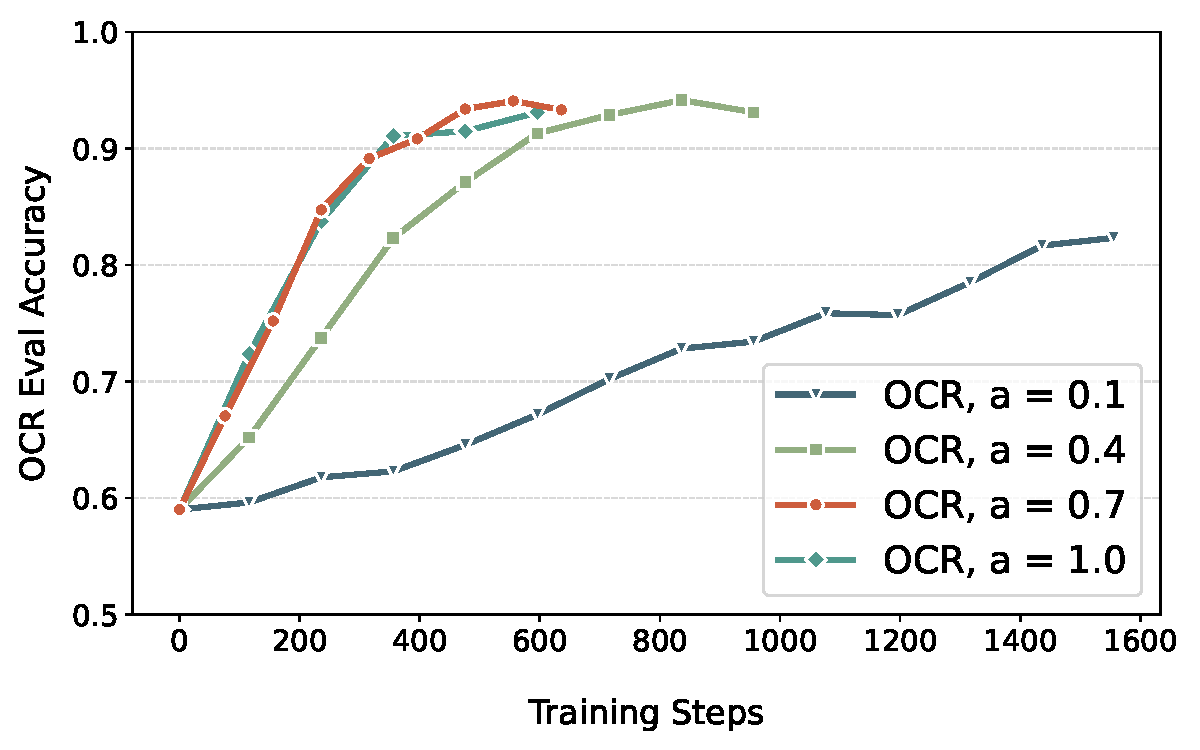
\includegraphics[width=\linewidth]{src/experiments/ablation_noise/exp1_ocr_ablation_noise.pdf}
    \vspace{-1.5em}
    \caption*{\footnotesize (b). Effect of Noise Level Ablation on the OCR}
  \end{minipage}
  % \begin{minipage}[t]{0.48\textwidth}
  %   \centering
  %   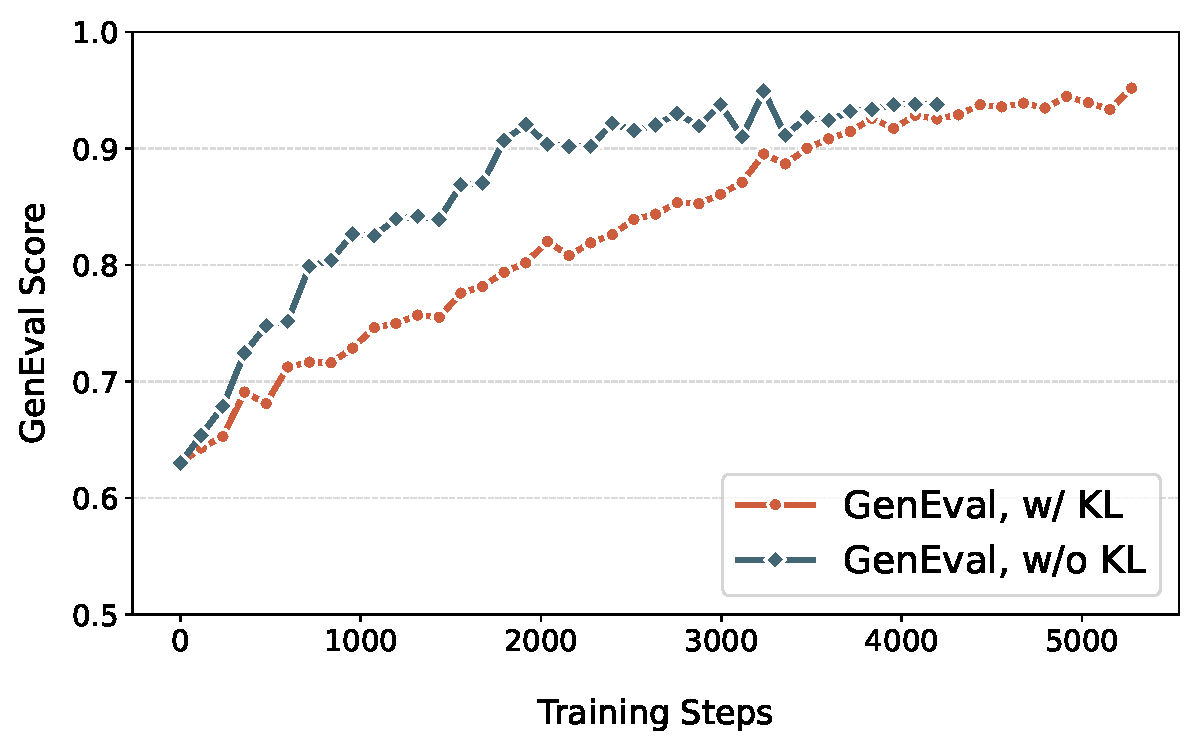
\includegraphics[width=\linewidth]{src/experiments/ablation_kl/exp3_geneval_ablation_kl.pdf}
  %   \vspace{-1.5em}
  %   \caption*{\footnotesize (b). Effect of KL‑Regularization on GenEval}
  % \end{minipage}
  % \vspace{1.5em}

  \caption{
  Ablation studies on our critical design choices. 
  \textbf{(a) Denoising Reduction}: Fewer denoising steps accelerate convergence and yield similar performance.
  % \textbf{(b) KL-Regularization}: KL penalty slows early training yet effectively suppresses reward hacking.
  \textbf{(b) Noise Level:} Moderate noise level ($a = 0.7$) maximises OCR accuracy, while too little noise hampers exploration.
  }
  \vspace{-2mm}
  \label{fig:exp_ablation}
\end{figure}

\paragraph{Effect of Group Size.}\label{sec:exp:group_number}
Figure~\ref{fig:abltion_groupsize} shows the effect of group size $G$ using PickScore as the reward function. When the group size was reduced to $G=12$ and $G=6$, training became unstable and eventually collapsed, whereas $G=24$ remained stable throughout the process. We observe that smaller group sizes produce inaccurate advantage estimates, increasing variance and leading to training collapse, a phenomenon also reported in~\cite{liu2025prorl,chen2025acereason}.

\paragraph{Generalization Analysis.}
Flow-GRPO demonstrates strong generalization on unseen scenarios from GenEval (Table~\ref{tab:geneval_unseen}). Specifically, it captures object number, color, and spatial relations, generalizing well to unseen object classes. It also effectively controls object count, generalizing from training on $2-4$ objects to generate $5-6$ or $12$ objects. Furthermore, Table~\ref{tab:t2i_comp_bench} shows Flow-GRPO achieves significant gains on T2I-CompBench++~\cite{T2i-compbench, huang2025t2i}. This comprehensive benchmark for open-world compositional T2I generation features object classes and relationships substantially different from our model's GenEval-style training data.

% \begin{table}[]
% \centering
%     \caption{\textbf{Flow-GRPO demonstrates strong generalization.} Unseen Obj.: Trained on 60 object classes, evaluated on 20 unseen classes. Unseen Attr. Binding: The model from Figure~\ref{fig:teaser} is evaluated on 10 unseen colors. Unseen Counting: The same model from Figure~\ref{fig:teaser}, initially trained to render 2, 3, or 4 objects, was evaluated on rendering 5 or 6.}
% \begin{tabular}{lccc}
% \toprule
% \multicolumn{1}{l}{} & Unseen Obj. & Unseen Attr. Binding & Unseen Counting \\ \midrule
% SD3-M                & 0.60            & 0.34              & 0.14            \\
% SD3-M+Flow-GRPO      & 0.83           & 0.57              & 0.45            \\ \bottomrule
% \end{tabular}
% \label{tab:geneval_unseen}
% \end{table}

\begin{table}[h]
\centering
\small
    \caption{{\bf T2I-CompBench++ Result.} This evaluation uses the same model presented in Table~\ref{tab:geneval}, which was trained on the GenEval-generated dataset.
The best score is in \colorbox{pearDark!20}{blue}.}
\resizebox{\linewidth}{!}{
\begin{tabular}{lccccccc}
\toprule
\textbf{Model} & \textbf{Color} & \textbf{Shape} & \textbf{Texture} & \textbf{2D-Spatial} & \textbf{3D-Spatial} & \textbf{Numeracy} & \textbf{Non-Spatial} \\ \midrule
Janus-Pro-7B~\cite{chen2025janus}  & 0.5145 & 0.3323 &0.4069 & 0.1566 & 0.2753 & 0.4406 & 0.3137 \\
EMU3~\cite{wang2024emu3} & 0.7913 & 0.5846 & \colorbox{pearDark!20}{0.7422} & — & — & — & — \\
FLUX.1 Dev~\cite{flux2024}         & 0.7407 & 0.5718 & 0.6922 & 0.2863 & 0.3866 & 0.6185 & 0.3127 \\
SD3.5-M~\cite{sd3}           & 0.7994 & 0.5669 & 0.7338 & 0.2850  & 0.3739 & 0.5927 & 0.3146 \\
\textbf{SD3.5-M+Flow-GRPO} & \colorbox{pearDark!20}{0.8379} & \colorbox{pearDark!20}{0.6130} & 0.7236 & \colorbox{pearDark!20}{0.5447} & \colorbox{pearDark!20}{0.4471} & \colorbox{pearDark!20}{0.6752} & \colorbox{pearDark!20}{0.3195} \\ \bottomrule
\end{tabular}
}
\vspace{-2mm}
\label{tab:t2i_comp_bench}
\end{table}

\begin{table}[h]
\centering
    \caption{\textbf{Flow-GRPO demonstrates strong generalization.} Unseen Objects: Trained on 60 object classes, evaluated on 20 unseen classes. Unseen Counting: Trained to render 2, 3, or 4 objects, and evaluated in two settings: rendering 5 or 6 objects, and rendering 12 objects.}
\resizebox{\linewidth}{!}{
\begin{tabular}{lccccccccc}
\toprule
\multirow{2}{*}{\textbf{Method}} & \multicolumn{7}{c}{\textbf{Unseen Objects}}                                              & \multicolumn{2}{c}{\textbf{Unseen Counting}} \\ \cmidrule(lr){2-8} \cmidrule(l){9-10} 
                        & \textbf{Overall} & \textbf{Single Obj.} & \textbf{Two Obj.} & \textbf{Counting} & \textbf{Colors} & \textbf{Position} & \textbf{Attr. Binding} & \textbf{5$-$6 Objects} &\textbf{12 Objects}        \\ \midrule
SD3.5-M                   & 0.64    & 0.96        & 0.73     & 0.53     & 0.87   & 0.26     & 0.47          & 0.13    & 0.02              \\
\textbf{SD3.5-M+Flow-GRPO}         & \colorbox{pearDark!20}{0.90}        & \colorbox{pearDark!20}{1.00}        & \colorbox{pearDark!20}{0.94}         & \colorbox{pearDark!20}{0.86}         & \colorbox{pearDark!20}{0.97}       & \colorbox{pearDark!20}{0.84}         & \colorbox{pearDark!20}{0.77}              & \colorbox{pearDark!20}{0.48}      & \colorbox{pearDark!20}{0.12}           \\ \bottomrule
\end{tabular}
}
\vspace{-2mm}
\label{tab:geneval_unseen}
\end{table}

% This structure emphasizes methodological generality while highlighting task-specific insights, ensuring reproducibility through hyperparameter transparency and ablation rigor.